\documentclass[a4paper]{article}
%Fonts 
\fontencoding{T1}
\usepackage{textcomp}
\usepackage{microtype}
\usepackage{mathpazo}
%\usepackage[oldstyle]{libertine}
%%\usepackage{libertinust1math}
%\usepackage[scaled=0.81]{beramono}


\usepackage{amsmath}
\usepackage{graphicx}
\usepackage{upquote}
\usepackage{listings}
\usepackage{xcolor}
\usepackage{siunitx}
\newcommand{\chezyunit}{\m\tothe{1/2}\per\s}

\usepackage{hyperref}
\usepackage{natbib}
\usepackage{asymptote}

\usepackage{parskip}
\setlength{\parindent}{0pt}

\usepackage{xsim}
\loadxsimstyle{layouts}

\DeclareExerciseHeadingTemplate{custom}
  {\section{\XSIMexpandcode{\XSIMtranslate{default-heading}}}}

\DeclareExerciseEnvironmentTemplate{custom}
  {%
    \IfInsideSolutionTF
      {\label{sol:\ExerciseID}}
      {\label{ex:\ExerciseID}}
    \subsection*
      {%
        \XSIMmixedcase{\GetExerciseName}%
        \IfInsideSolutionTF
          {
            to \GetExerciseParameter{exercise-name}%
            ~\GetExerciseProperty{counter}%
          }
          {%
            ~\GetExerciseProperty{counter}
            \GetExercisePropertyT{subtitle}
              { {\normalfont\itshape\PropertyValue}}%
          }%
      }
    \noindent\llap{%
      \footnotesize\sffamily
      \IfInsideSolutionTF
        {%
          \XSIMmixedcase{\GetExerciseParameter{exercise-name}}
          on page~\pageref{ex:\ExerciseID}.%
        }
        {%
          \XSIMmixedcase{\GetExerciseParameter{solution-name}}
          on page~\pageref{sol:\ExerciseID}.%
        }%
      \hspace*{\marginparsep}%
    }%
  }
  {}
\xsimsetup{
  exercise/template = custom ,
  solution/template = custom ,
  print-solutions/headings-template = custom
}




% \xsimsetup{
%   exercise/template=runin,
%   solution/template=runin,
%   solution/print=false% Change to false to disable printing solutions
% }

\title{River flow and morphology -- PC practical 1}
\author{B. Vermeulen}
%\qformat{\textbf{Exercise \thequestion} \hfill}

\newcommand{\der}[2]{\dfrac{\mathrm{d}#1}{\mathrm{d}#2}}
\newcommand{\pder}[2]{\dfrac{\partial#1}{\partial!2}}
\newcommand{\pdder}[2]{\dfrac{\partial^2#1}{\partial#2^2}}

\definecolor{codegreen}{rgb}{0,0.6,0}
\definecolor{codegray}{rgb}{0.5,0.5,0.5}
\definecolor{codepurple}{rgb}{0.58,0,0.82}
\definecolor{backcolour}{rgb}{0.95,0.95,0.92}

\lstdefinestyle{mystyle}{
    backgroundcolor=\color{backcolour},
    commentstyle=\color{codegreen},
    keywordstyle=\color{blue},
    numberstyle=\tiny\color{codegray},
    stringstyle=\color{codepurple},
    basicstyle=\ttfamily\footnotesize,
    breakatwhitespace=false,
    breaklines=true,
    captionpos=b,
    keepspaces=true,
    numbers=left,
    numbersep=5pt,
    showspaces=false,
    showstringspaces=false,
    showtabs=false,
    tabsize=2,
}

\lstset{
  style=mystyle, 
  language=Matlab,
  deletekeywords={ans, xlabel, ylabel, plot, legend, title, close, all},
  morekeywords={*, classdef, properties, methods}
}

% hyperref settings
\colorlet{link}{black!60!red}
%\colorlet{link}{black}
\hypersetup{
    unicode=false,          % non-Latin characters in Acrobat's bookmarks
    pdftoolbar=true,        % show Acrobat's toolbar?
    pdfmenubar=true,        % show Acrobat's menu?
    pdffitwindow=false,     % window fit to page when opened
    pdfstartview={FitH},    % fits the width of the page to the window
    pdftitle={River flow and morphology},    % title
    pdfauthor={HWM},     % author
    pdfcreator={HWM},   % creator of the document
    pdfproducer={HWM}, % producer of the document
    pdfnewwindow=true,      % links in new PDF window
    colorlinks=true,       % false: boxed links; true: colored links
    linkcolor=link,          % color of internal links (change box color with linkbordercolor)
    citecolor=link,        % color of links to bibliography
    filecolor=link,      % color of file links
    urlcolor=link,           % color of external links
}

\begin{document}
\maketitle
\tableofcontents

\section{Introduction}
\label{sec:intro}
This computer practical is part of the course ``River flow and morphology''. This practical contributes to the understanding of steady, non uniform dynamics of river systems by working through a number of river engineering problems. At the end of this practical students are expected to be able to: 
\begin{enumerate}
  \item Perform basic mathematical operations and simple programming tasks in MATLAB
  \item Make use of object oriented classes in MATLAB
  \item Run a backwater computation by setting the proper variables and setting the right boundary conditions
  \item Show at what spatial scales backwater curves occur and what affects these spatial scales
  \item Combine backwater computations by imposing the proper boundary conditions
  \item Predict how changes to the river system affect the backwater hydrodynamics
  \item Predict the position of a hydraulic jump, and how backwaters interact at a hydraulic jump
\end{enumerate}

In the first part of the practical you will familiarize with the basic syntax of MATLAB (\autoref{sec:matlab_tutorial}).
Subsequently the Backwater class is introduced that you can use to perform backwater calculations.
The practical continues with an exercise in which you will try to reproduce all types of backwater.
Afterwards, an example is shown on how different backwaters can be combined, when dealing with different river reaches. 
Finally you will work on a problem, that you can solve by combining different backwater curves.
Eventually you will work on the case of a hydraulic jump.
 
\section{MATLAB: a very short introduction}
\label{sec:matlab_tutorial}
\subsection{Vectors and matrices}
Open MATLAB, you will see the following window:

\begin{figure}
	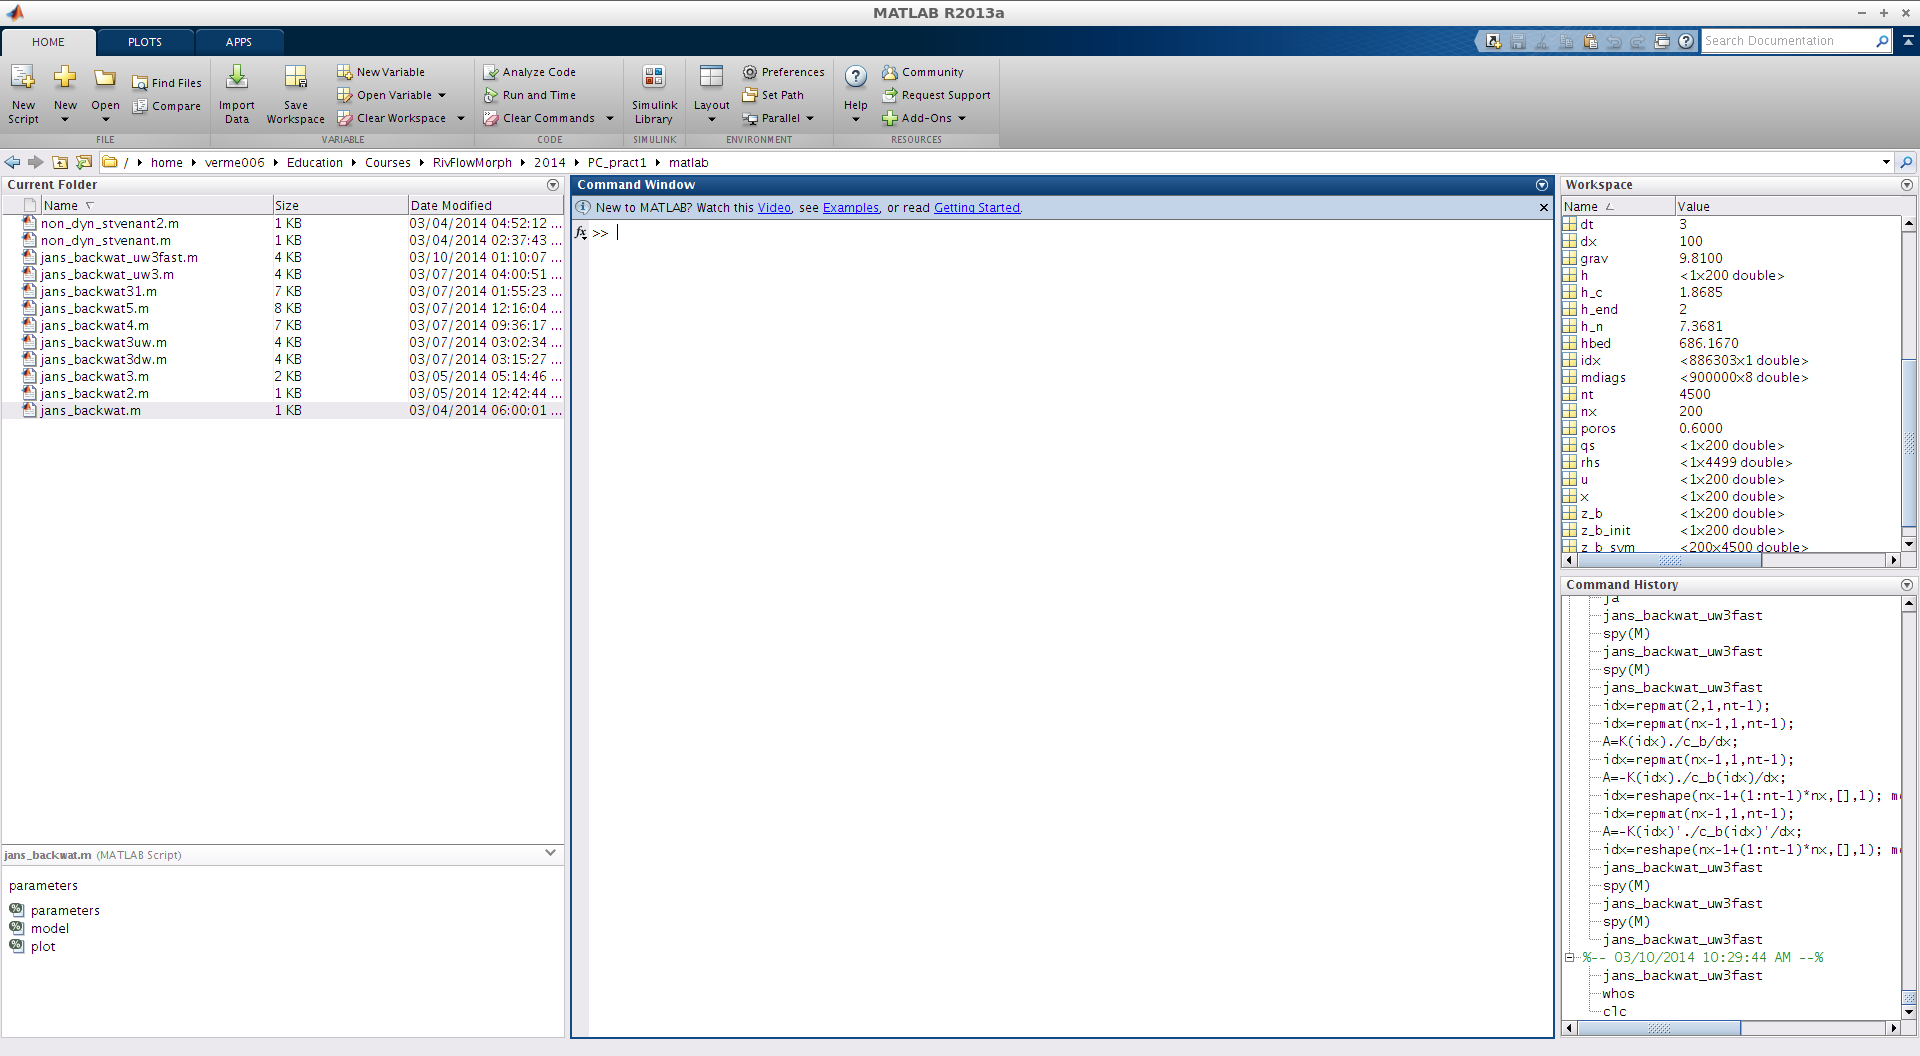
\includegraphics[width=\linewidth]{matlab_start.png}
  \caption{The MATLAB window.}
\end{figure}

In the command window you can type commands to MATLAB.
We start by making a simple variable:
\begin{lstlisting}
	>> a=5
  a =
	    5
\end{lstlisting}
We can also create a row vector:
\begin{lstlisting}
	>> b=[1 3 4]
	b =
	     1     3     4
\end{lstlisting}
Or a column vector:
\begin{lstlisting}
	>> c=[5;4;3]
	c =
	     5
	     4
	     3	
\end{lstlisting}
Please note that you can see the variables in the ``Workspace'' window.
\begin{figure}
  \centering
  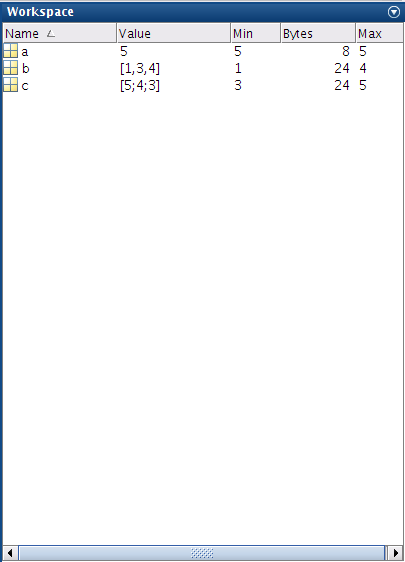
\includegraphics[width=.5\linewidth]{Workspace.png}
	\caption{Variables in your workspace.}
\end{figure}
So white spaces concatenate numbers or variables horizontally and semi-colons vertically.
This way you can also construct a matrix:
\begin{lstlisting}
>> d=[b; 5 6 8; a a a]
d =
     1     3     4
     5     6     8
     5     5     5
\end{lstlisting}

\begin{exercise}
  Try yourself to construct the following matrix and name it \lstinline=e=:
    \begin{equation}
    	\begin{pmatrix}
    		1 & 2 & 3 \\
    		6 & 5 & 3 \\
    		0 & 0 & 1 
    	\end{pmatrix}
    \end{equation}
\end{exercise}
\begin{solution}
  \begin{lstlisting}
>> e = [1 2 3; 6 5 3; 0 0 1]

e =

     1     2     3
     6     5     3
     0     0     1

>>
  \end{lstlisting}
\end{solution}

The content of a variable can be seen in MATLAB by typing the variable name:
\begin{lstlisting}
>> d
d =
     1     3     4
     5     6     8
     5     5     5
>>
\end{lstlisting}
When you put a semi-colon behind any statement all output to the window is suppressed:
\begin{lstlisting}
>> d;
>>
\end{lstlisting}

You can use the command \lstinline=whos= to see what is in your workspace (or look in the Workspace window):
\begin{lstlisting}
>> whos
  Name      Size             Bytes  Class     Attributes

  a         1x1                  8  double              
  b         1x3                 24  double              
  c         3x1                 24  double              
  d         3x3                 72  double              
  e         3x3                 72  double              
  f         1x101              808  double              

>>
\end{lstlisting}
In the left column you see the names of the variables. In the second column you can see the ``size'' of the variables. All variables, including scalars and vectors have two dimensions.
The first number indicates the number of rows and the second one, the number of columns. The variable \lstinline=a= has size 1x1 and is therefor a scalar. \lstinline=b= has one row and three columns: a row vector. \lstinline=c= is a column vector and \lstinline=e= is a 3x3 matrix. The third column indicates the number of bytes a variable occupies in memory. Since all variables are of type (column 4) double (double precision floating point) they occupy 8 bytes per element. 
Another way to view your variables is by double-clicking them in the Workspace window. This will open a spreadsheet-like view, showing the values in the variables (Figure~\ref{fig:vareditor}).

\begin{figure}
  \centering
  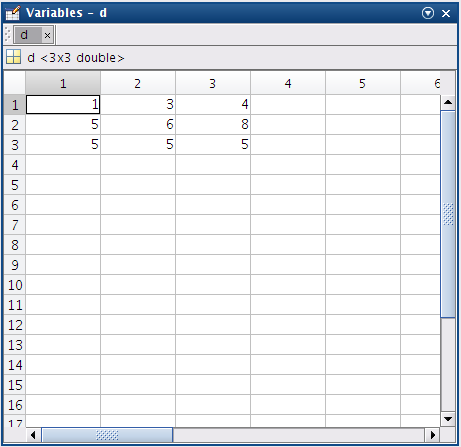
\includegraphics[width=.5\linewidth]{vareditor.png}
    \caption{The variable editor window.}
    \label{fig:vareditor}
\end{figure}

Apart from manually typing variables, MATLAB offers a great number of function to help in the creation of variables. We will discuss the most common ones here:
Suppose you want to make a vector containing: $(0, 3, 6, 9, \ldots, 300)$. This is easily done as follows:
\begin{lstlisting}
    >> f=0:3:300;
    >> 
\end{lstlisting}
Similarly you can create a column vector:
\begin{lstlisting}
    >> a=(0:3:300)';
    >> 
\end{lstlisting}
Now the same statement is surrounded by parentheses\footnote{Without the parentheses we would just transpose the 300, and the result would be the same row vector as before.} and there is an apostrophe (\lstinline='=) behind it. This indicates that the matrix should be transposed.
If you want to create a row vector with 200 numbers in the interval $[0,\pi]$ you can use:
\begin{lstlisting}
    >> a=linspace(0, pi, 200);
    >>
\end{lstlisting}

\begin{exercise}
  Can you create the same vector, but this time as a column vector?
\end{exercise}
\begin{solution}
  \begin{lstlisting}
    >> a=linspace(0, pi, 200)'; % Notice the prime 
    >>
  \end{lstlisting}
\end{solution}

You can reference specific elements by using indexing. Here a few examples:
\begin{lstlisting}
>> c
c =
     5
     4
     3
\end{lstlisting}
Show me the second element of \lstinline=c=
\begin{lstlisting}
>> c(2)
ans =
     4
\end{lstlisting}
Show me \lstinline=d= and after that the element on the first row and third column:
\begin{lstlisting}
>> d
d =
     1     3     4
     5     6     8
     5     5     5
>> d(1,3)
ans =
     4
\end{lstlisting}
Show me all element in second column of \lstinline=d=
\begin{lstlisting}
>> d(:,2)
ans =
     3
     6
     5
\end{lstlisting}
Show me all element in third row of \lstinline=d=
\begin{lstlisting}
>> d(3,:)
ans =
     5     5     5
\end{lstlisting}
Show me all element of \lstinline=d=
\begin{lstlisting}
>> d(:)
ans =
     1
     5
     5
     3
     6
     5
     4
     8
     5
\end{lstlisting}
Notice that in the last statement all elements are placed in a column. MATLAB collects the elements from \lstinline=d= column by column. 
When using seperate indices for each dimension, we call the indices subscripts, otherwise we call them single indices.
It is also possible to use the keyword \lstinline=end= in the subscripts or linear indices, which always refers to the last element in a specific dimension (for subscripts) or the last element of the entire array (for single indexing).

Apart from manually referencing elements you can use other variable with integers to reference elements:
\begin{lstlisting}
>> idx=[1 3]
idx =
     1     3
>> d(idx,1)
ans =
     1
     5
>> d(1,idx)
ans =
     1     4
>> d(idx,idx)
ans =
     1     4
     5     5
>> 
\end{lstlisting}
Another way to index variables is called logical indexing. In this case elements are referenced by the `true' values in a binary vector. This is particularly useful if you, for instance, would like to change all values in a vector that meet some criteria. We may want to add 1 to all elements in \lstinline=d= smaller than 4:
\begin{lstlisting}
>> d
d =
     1     3     4
     5     6     8
     5     5     5
>> d(d<4)=d(d<4)+1
d =
     2     4     4
     5     6     8
     5     5     5
>> 
\end{lstlisting}

A lot more information on creation and manipulation of matrices can be found in the MATLAB help \footnote{The MATLAB help is extremely useful, so use it a lot. Whenever you are thinking of making a function to do some job, spend first some time to look in the help if there is already a function that can do the job for you. Big chance such function is already there.}:
\begin{lstlisting}
>> web([docroot '/matlab/matrices-and-arrays.html'])
>>
\end{lstlisting}

You can delete all variables with the command:
\begin{lstlisting}
>> clearvars
>>
\end{lstlisting}

\subsection{Operations with vectors and matrices}
A nice feature of MATLAB is that you can perform easily operations with vectors and matrices. An important distinction to make when talking about operations with vectors and matrices is whether we are performing an element-wise operation or a matrix operation. I will explain the difference in the following example. We start with two 3x3 matrices:
\begin{lstlisting}
>> a=eye(3)
a =
     1     0     0
     0     1     0
     0     0     1
>> b=magic(3)
b =
     8     1     6
     3     5     7
     4     9     2
>> 
\end{lstlisting}
The first matrix is an identy matrix, the second one is a matrix whose columns and rows sum up to the same number.
We can now multiply these two matrices in two ways: with a matrix multiplication and with an element-wise multiplicaton:
\begin{lstlisting}
>> a*b
ans =
     8     1     6
     3     5     7
     4     9     2
>> a.*b
ans =
     8     0     0
     0     5     0
     0     0     2
>> 
\end{lstlisting}
The result is very different. In the first case the two matrices were multiplied (\lstinline=*=). In the second case the elements of the two matrices were multiplied (\lstinline=.*=). In general when an operator, \lstinline=*= in this case, is preceded by a \lstinline=.=, an element-wise operation is performed. A similar example:
\begin{lstlisting}
>> b^2
ans =
    91    67    67
    67    91    67
    67    67    91
>> b.^2
ans =
    64     1    36
     9    25    49
    16    81     4
>>
\end{lstlisting}


\subsection{Using script files}
Until now we have been typing all commands directly in the command window. It is often useful to store all commands in a script file. Matlab script-files have the extension \lstinline=.m=. You can start editing a new script file:
\begin{lstlisting}
>> edit example1.m
>>
\end{lstlisting}
This will open a new script file named \lstinline=example1.m=. It is a good habit to start scripts with a \lstinline!clearvars! command to clean everything in the workspace. This way we make sure that no pre-existing variables in the Workspace will influence our script. You can run a complete script pressing ``\lstinline!F5!''. If you want to run only some lines, select them, and press ``\lstinline!F9!''. This will paste the line in the command window. Another way to run the script is to type  the name of the script without extension on the command line:
\begin{lstlisting}
>> example1
>>
\end{lstlisting}
When editing a script, MATLAB will  warn you whenever it thinks (and usually it is right) you are making a mistake. It will highlight this like a spelling corrector does. When hovering over the error with your mouse, a tool-tip will tell you what is wrong.
When a line is not terminated with a semicolon, a warning is shown, because running the script may produce a huge amount of output to the screen.
\begin{figure}
  \centering
  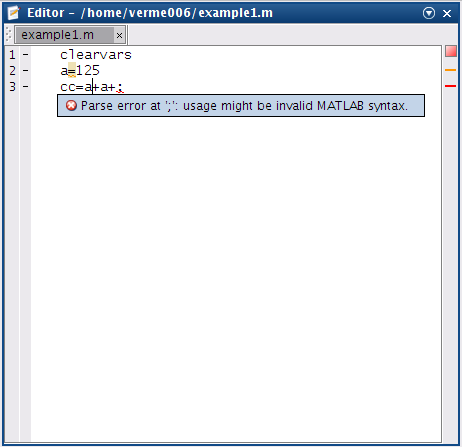
\includegraphics[width=.5\linewidth]{script.png}
    \caption{Script editor showing a warning and an error. Hovering over the place where the error is generated shows a tool-tip informing us about what caused the error. On the first line a warning is given because the statement is not terminated by a semicolon. The script still functions but may produce a lot of output to the command windows.}
    \label{fig:script}
\end{figure}
Comments can be added anywhere in the script using a \lstinline!%! sign. 

\begin{exercise}
    Create a script that does the following:
    \begin{itemize}
        \item Create a column vector with numbers from 0 to 400
        \item Multiply all odd numbers in the vector with 2
        \item Compute the sinus of the squared of the natural logarithm of all elements in the vector
        \item Save the script
    \end{itemize}
\end{exercise}
\begin{solution}
  Open a new file named \lstinline{weird_func.m} in the editor and type:
  \lstinputlisting{matlab/weird_func.m}
  Press \lstinline{Ctrl+S} to give the script a name and save it.
\end{solution}

\subsection{Plotting}
In this last part we will make some plots, but first we need to generate some data.
\begin{exercise}
  Empty your workspace and create a vector \lstinline!x! with 100 elements in the range $[0, 2\pi]$. Create a vector \lstinline!y! which contains the values $\sin^2(x)-\cos(x)$.
\end{exercise}
\begin{solution}
  \begin{lstlisting}
>> clearvars % empty the workspace
>> x = linspace(0, 2*pi, 100);
>> y = sin(x).^2-cos(x);
  \end{lstlisting}
\end{solution}
Now we will plot the result:
\begin{lstlisting}
>> plot(x,y)
>>
\end{lstlisting}
You should see something similar to Figure~\ref{fig:plot}. Now play with the tools (zoom in, zoom out, pan, etc.) in the figure window to familiarize with them.
\begin{figure}
  \centering
  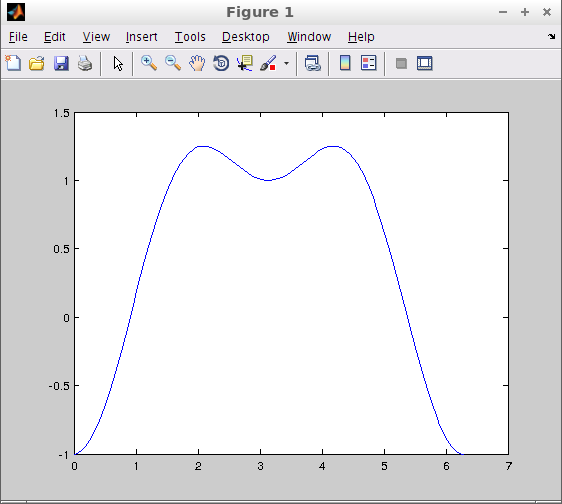
\includegraphics[width=.5\linewidth]{plot.png}
    \caption{Your first plot in MATLAB.}
    \label{fig:plot}
\end{figure}

\begin{exercise}
  Now, using the help of MATLAB (\lstinline!help plot!), find out how to make the plot in Figure~\ref{fig:plotred}.
\end{exercise}
\begin{solution}
  \begin{lstlisting}
>> plot(x, y, 'rx-', 'LineWidth', 2)
  \end{lstlisting}
\end{solution}
\begin{figure}
  \centering
  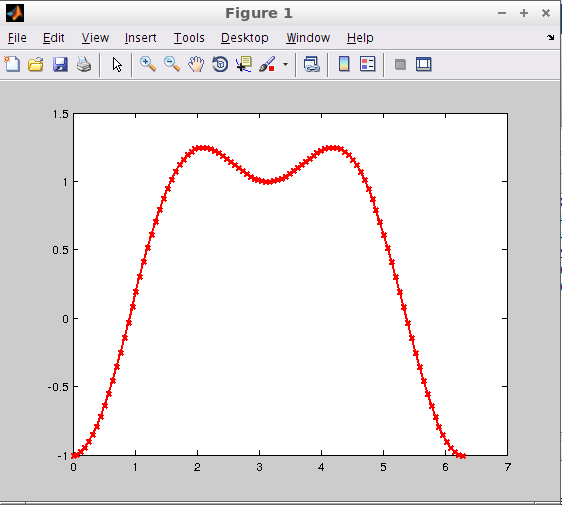
\includegraphics[width=.5\linewidth]{plot_red.png}
    \caption{Try to reproduce this plot.}
    \label{fig:plotred}
\end{figure}
Of course, no figure is complete without axis labels, a title and a legend:
\begin{lstlisting}
>> xlabel('x (-)')
>> ylabel('y (-)')
>> title('Red line')
>> legend('sin^2(x)-cos(x)')
>> 
\end{lstlisting}

When plotting from a script it can be usefull to include a \lstinline!close all! statement to close all figures previously made. This avoids that your script will start plotting in ``old'' figures.

\begin{exercise}
    \begin{enumerate}
        \item Make a new script called \lstinline!plot_bed_slope.m! to contain everything from this question.
        \item Define a slope (\lstinline!So!) and a length of a river reach (\lstinline!L!). Use comments to explain the meaning of the variables.
        \item Construct a two element vector with start and end of reach.
        \item Compute the bed-elevation (\lstinline!z_b!) given the variables you just defined.
        \item Make a nice figure of the bed you just computed.
        \item Play around with the parameters, changing slope, length etc. and look how the plot changes (by rerunning the script).
    \end{enumerate}
\end{exercise}

\begin{solution}
  Open a new script in the editor and save it as \lstinline!plot_bed_slope.m!. Type the following:
  \lstinputlisting{matlab/plot_bed_slope.m}
\end{solution}


\subsection{Functions}
In MATLAB it is also possible to define functions. These are similar to scripts, but allow to define specific inputs and they return some outputs. Functions are pieces of code designed to perform a specific task. A function might look as follows:
\begin{lstlisting}
  function c = add_up(a,b)

  c=a+b;
\end{lstlisting}
You can create a function in the same way you create a script. When you save the function you should take care that you save it with the same name as the function name (in this case \lstinline=add_up=).

Once saved, the function can be called as follows:
\begin{lstlisting}
>> add_up(1,2)

ans =

     3

\end{lstlisting}
Note that the variables \lstinline=a= and \lstinline=b= defined in the function are local to the function, i.e. changing the value of \lstinline=a= outside of the function will not affect the value of a inside the function.

MATLAB functions can also have multiple outputs, e.g.
\begin{lstlisting}
function [s, d] = add_and_subtract(a, b)

s = a + b;
d = a - b;
\end{lstlisting}
When the function returns multiple results, you can get the results as follows:
\begin{lstlisting}
>> [c, e] = add_and_subtract(a,b);
\end{lstlisting}

\begin{exercise}
  Create a function that given a slope and a vector with $x$ position returns the bed-level elevation, assuming the elevation is 0 for $x=0$
\end{exercise}
\begin{solution}
After creating a file with the name of the function you want to create (in this case \lstinline=bed_slope.m= add the following content:
\lstinputlisting[]{matlab/bed_slope.m}
\end{solution}

\subsection{Classes and objects}
In this last part we will introduce the concept of classes and objects. Classes can be very usefull when we want to combine data and functions that conceptually ``belong together''. This section only provides a very brief introduction to classes and only ``handle'' classes. For more details on classes see the MATLAB manual.

So, suppose that we want to write a class that represents a piece of river. Such a river has certain properties, such as discharge, slope and roughness and length. Furthermore we want this river class to perform some operations, like computing the bed elevation, as we saw before. We can define a class as follows in the editor:
\begin{lstlisting}
classdef River < handle

end
\end{lstlisting}
The file needs to be saved with the same name as the class to be used, i.e. \lstinline{River}. Now, we can add so-called properties:
\begin{lstlisting}
classdef River < handle
  properties(Constant)
    g=9.81
  end
  properties
    slope=1e-4
    discharge=1000
    chezy=50
  end
end
\end{lstlisting}
Notice that we have two kind of properties (there are many more types you can define, but this will do for now), a constant property (you cannot modify this one) and three normal properties. For all properties we defined default values.

Now we have defined a class, we can create an object of the class. This means that we create a variable of the type \lstinline=River=:
\begin{lstlisting}
>> R=River

R =

  River with properties:

            g: 9.8100
        slope: 1.0000e-04
    discharge: 1000
        chezy: 50

\end{lstlisting}
You can change the properties of the class:
\begin{lstlisting}
>> R.slope=1e-3;
\end{lstlisting}
An important property of handle classes in MATLAB is that if we copy the class, e.g. \lstinline|R_copy=R|, these copies point to the same object. That means that if I change a property of \lstinline=R_copy= the property of \lstinline=R= also changes. Both variables point to the same object.

No we have a class, but this class is still pretty useless. Let's add some functionality. We might want to compute the critical slope of the river. For this we need a function. We can define a function within the class, which is called a ``method'' of the class:
\lstinputlisting[linerange={1-8,10-14,18-19}]{matlab/River.m}

We can now compute the critical slope as:
\begin{lstlisting}
>> R.critical_slope

ans =

    0.0039

\end{lstlisting}
If we change the roughness, the critical slope will change accordingly:
\begin{lstlisting}
>>  R.chezy=70;
>>  R.critical_slope

ans =

    0.0020

\end{lstlisting}

\begin{exercise}
  Extend the river class with an \lstinline=L= property to hold the length of the river and a method that computes the bed elevation between $[0, L]$ at 15 points.
\end{exercise}
\begin{solution}
\lstinputlisting{matlab/River.m}
\end{solution}


\section{The Backwater class}
\label{sec:backwater_class}

\subsection{Introduction}
Now that you familiarized with MATLAB, we will start working with the \lstinline=Backwater= class that was created for this practical. This class allows to perfrom backwater calculations for pieces of a river. We will start by looking at one river reach, and after that we will continue by combining different river reaches together.

First of all, you need to download the backwater class from brigthspace and place the \lstinline=Backwater.m= file in you working folder. You can start by creating a backwater object:
\begin{lstlisting}
B=Backwater;
\end{lstlisting}
To learn how to use the object you can run
\begin{lstlisting}
doc Backwater
\end{lstlisting}
This will open a window with the documentation of the Backwater class. You can click on the properties and methods names to get explanation about what the properties are and what methods do. Do not worry if you do not understand all the details, many of the options have to do with the computations needed to solve the backwater equation.
\begin{figure}[h]
  \centering
  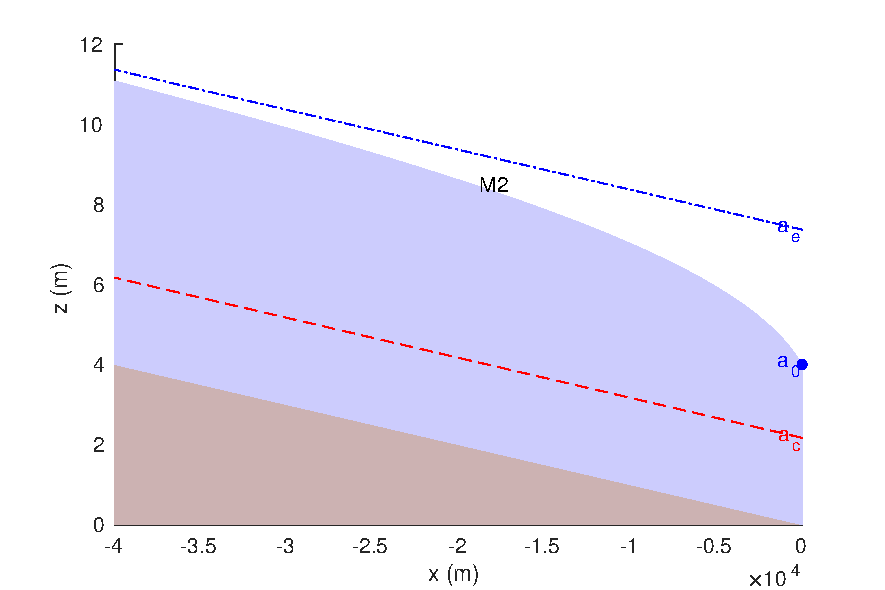
\includegraphics{m2_curve.pdf}
  \caption{Plotting the \lstinline{Backwater} object}
  \label{fig:m2_curve}
\end{figure}

A nice feature of the Backwater class is that you can easily make a nice plot of the current situation by running:
\begin{lstlisting}
plot(B) % B is a Backwater object
\end{lstlisting}
This will generate a figure as in \autoref{fig:m2_curve}. The figure shows a longitudinal profile of the river, with the bed and the water surface. The blue dash-dotted line indicates the equilibrium depth and the red, dashed line indicates the critical water depth. At the left boundary the $a_0$ is inidicated.
\begin{exercise}
  What is the meaning of $a_e$ $a_c$ and $a_0$? Explain the meaning in terms of the underlying physics.
\end{exercise}

\begin{solution}
    $a_e$ is the equilibrium depth. At this depth we have uniform flow and gravity force and friction force exactly balance each other.
    $a_c$ is the critical depth. At this depth the flow is critical and the Froude number is equal to 1.
    $a_0$ is the boundary condition. When this deviates from the equilibrium depth a backwater curve develops
\end{solution}

\begin{exercise}
  What is the meaning of $S_c$?
\end{exercise}

\begin{solution}
    This is the critical slope. At this slope the equilibrium depth is equal to the critical depth. If a river's slope is larger we have a steep slope which features a supercritical flow in equilibrium. A lower slope results in a mild slope where a subcritical flow occurs in equilibrium conditions.
\end{solution}
Next to a number of quite obvious properties of the \lstinline{Backwater} object, there are also a few that require a bit more explanation:
\begin{itemize}
  \item \lstinline{x_end} indicates the ending $x$ coordinate for the backwater computation that always starts at $x0$. 
  \item \lstinline{x_target} is a read only property that gives an indication of a possible value for \lstinline{x_end}. 
\end{itemize}
The reason why the object is suggesting a possible ending coordinate is that sometimes this is not so obvious and you might need a bit of help.

\subsection{Making all backwater curve types}
The curve that you produced with the \lstinline{Backwater} object is an M2-curve. You can find this curve also in figure 4.3 on page 76 of the lecture notes. Figures 4.3 to 4.5 in the lecture notes show all the types of backwater curves that can develop.

\begin{exercise}
  Try to reproduce all types of backwater curves modifying the properties of the \lstinline{Backwater} object and make a plot of the curve. Note: make use of the \lstinline=x_target= property to set right length and direction of solution.
\end{exercise}

\begin{solution}
    \lstinputlisting{matlab/make_backwater_curves.m}
\end{solution}

\begin{exercise}
  Pay attention to the spatial scales of the curve you produced. Can you discover some kind of pattern in the spatial scale of the backwater curves?
\end{exercise}

\begin{solution}
    Mild slopes have long backwaters. Steep slopes have smaller backwaters, Horizontal and Adverse also have relatively short backwaters. Supercritical conditions also result in much smaller spatial scales for the backwater curves.
\end{solution}

\begin{exercise}
  Even though you use the same bed slope, for some curves the bed seems to plot horizontal and for some you can clearly see the slope. Explain what causes this difference in the plots.
\end{exercise}

\begin{solution}
    The reason has all to do with scale. When the backwater is occurring at a small scale the elevation change will be minimal over small distances.
\end{solution}

\section{Combining backwater curves}

\subsection{The example in the lecture notes revisited}
\label{sec:combining_backwaters}
In this section you will learn how backwater curves can be combined. As an example we will try to reproduce the example in the lecture notes in Section 4.1.6 about a river widening. In the example, a part of the river is being widened. In Figure 4.6 of the lecture notes you can see that by defining the section AB where river widening will occur, we are actually subdividing the river in three pieces:
\begin{enumerate}
  \item An upstream part
  \item The section that is being widened
  \item A downstream section
\end{enumerate}
In MATLAB we will need one \lstinline{Backwater} object for each river reach.
For this we construct an array of three Backwater objects:
\begin{lstlisting}
R(3)=Backwater; % River has three pieces
\end{lstlisting}
We will assume that the \lstinline{R(1)} is the upstream piece, \lstinline{R(2)} is the middle reach and \lstinline{R(3)} the downstream reach.
These object still contain the wrong values for discharge, slope, etc., so we will start by setting the right properties (we do so for the situation before the widening, so all reaches have the same width):
\begin{lstlisting}
[R(:).So]=deal(1e-4); % set the slope
[R(:).Chez]=deal(50); % set the roughness
[R(:).b]=deal(200); % set the width
[R(:).Q]=deal(800); % set the width
\end{lstlisting}
OK, this might look a bit strange. Let's have a closer look at this syntax: the part left to the equal sign \lstinline{[R(:).So]} is actually the same as writing \lstinline{[R(1).So, R(2).So, R(3).So]}. Looking at this like this you can see that we are actually assigning to output of the function right of the equal sign to the \lstinline{So} property of each object. The part left of the equal sign \lstinline{deal(1e-4)} calls the function \lstinline{deal}. This function gets the input \lstinline{So} and distributes it over the outputs. For the left hand side we might also have written \lstinline{[1e-4, 1e-4, 1e-4]}. So, putting it all together the first line is the same as \lstinline{[R(1).So, R(2).So, R(3).So]=[1e-4, 1e-4, 1e-4]}. The syntax above saves a lot of typing.

Now that we assigned the properties of the reaches, we need to get the geometry right. Now all the river reaches start and end at the same $x$ coordinate. This of course is not what we want. We will change the \lstinline{x0} and \lstinline{x_end}. Since the length of the upstream and downstream pieces are not given in the lecture notes we will make these \SI{20}{\km} and \SI{5}{\km}, respectively. Furthermore, we also need to make sure that the bed of the two usptream reaches does not start at $z_b=0$ elevation but at the elevation at which the downstream reach ends. For this reason we will also change the \lstinline{zb0} property:
\begin{lstlisting}
R(3).x0=0;

%Let's assume that the downstream reach has a length of 5 km, the we have:
R(3).x_end=-5e3;

% The end of the downstream piece is the start of the middle piece:
R(2).x0=R(3).x_end;
R(2).zb0=R(3).bed_level(end); % this method computes the bed elevation at x0 and x_end

% This piece has a length of 20 km so:
R(2).x_end=R(2).x0-20e3;

% Now we define the most upstream piece:
R(1).x0=R(2).x_end;
R(1).zb0=R(2).bed_level(end);

% Let's make this piece also 20 km:
R(1).x_end=R(1).x0-20e3;
\end{lstlisting}

\begin{exercise}
  If you consider that the boundary condition is always imposed at $x=x0$, what implicit assumption did we make about the type of flow by defining the geometry as we did in the above lines?
\end{exercise}

\begin{solution}
    The \lstinline|x_end| property was set to a negative value, meaning that the computation is done in upstream direction. This means that we assumed the flow to be subcritical. For supercritical flow we'd use a positive \lstinline|x_end|.
\end{solution}

The last thing that we need to do is set the right boundary condition. Since we start with the equilibrium situation, we will set the boundary depth equal to the equilibrium depth:

\begin{lstlisting}
[R(:).a0]=deal(R(:).a_equilibrium); % set the boundary depth
\end{lstlisting}

Now that we have everything set, we will make a first plot of the initial situation:
\begin{lstlisting}
plot(R)
\end{lstlisting}

\begin{figure}[h]
  \centering
  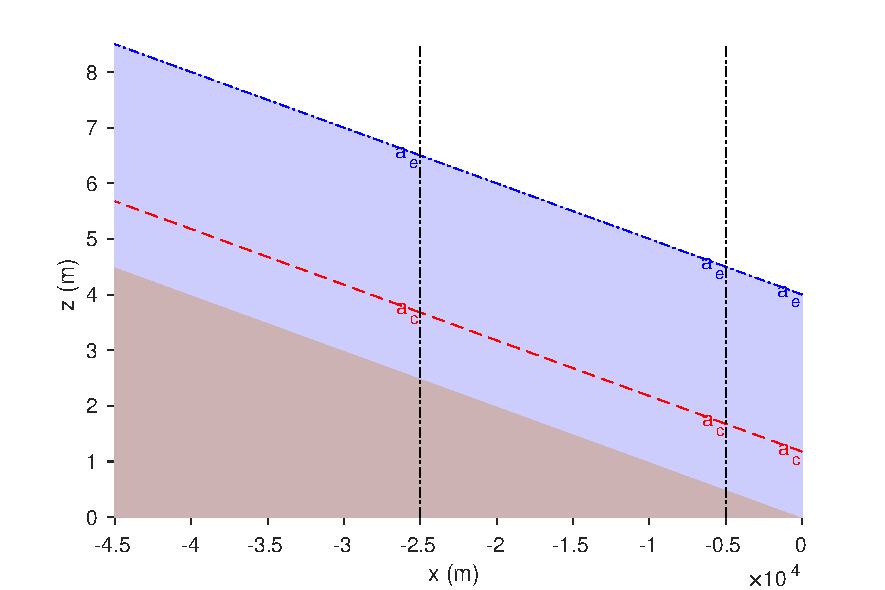
\includegraphics{widening_initial.pdf}
  \caption{Initial situation, before river widening. All river reaches are in equilibrium}
  \label{fig:widening_initial}
\end{figure}
If everything went well, you should get a figure similar to \autoref{fig:widening_initial}.

Now we can change the width in the middle reach:
\begin{lstlisting}
R(2).b=220;
\end{lstlisting}
If we plot the object after this change, we can see that a backwater is computed in the middle reach. For this reach, the boundary condition is still at the old equilibrium depth, which is right, since at the downstream end nothing changed. The equilibrium depth in the middle reach, however, changed, and as a result a backwater developed. At the upstream part of the middle reach, however, there is a jump in water level, which is not realistic. This is because we still need to set the boundary condition for the upstream part. The boundary condition for the upstream part is given by the depth and the upstream end of the middle reach. We can get that depth by using the method \lstinline{solve} that gives us the all the depths along the reach:
\begin{lstlisting}
[x,a]=R(2).solve; % this computes depths a at the location x
R(1).a0=a(end); % the last depth, i.e. at x=xend will be the downstream bc for the upstream reach
figure % we make a new figure
plot(R) % plot the result
\end{lstlisting}
This produces \autoref{fig:widening_final}.

\begin{figure}[h]
  \centering
  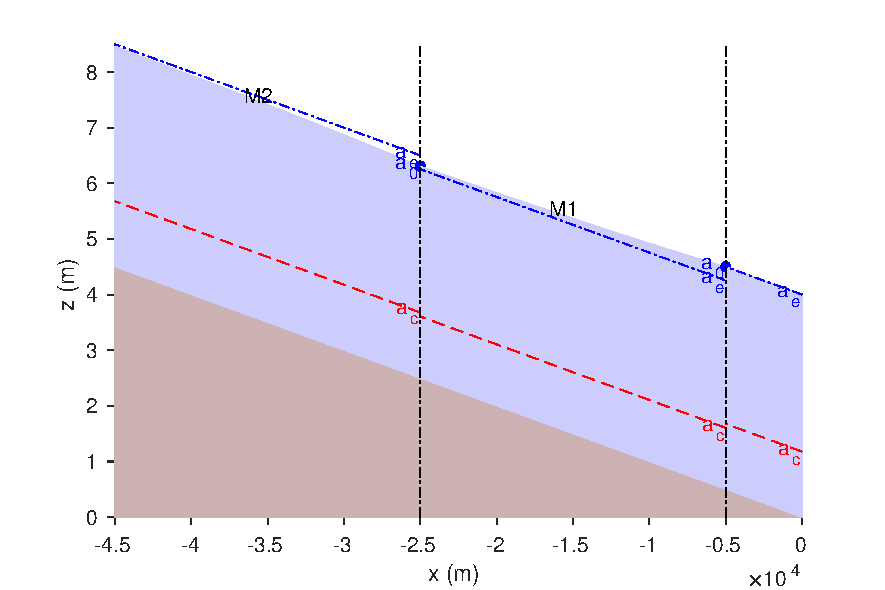
\includegraphics{widening_final.pdf}
  \caption{Final situation after river widening.}
  \label{fig:widening_final}
\end{figure}

\begin{exercise}
  How do the results of the computed backwater compare with the results obtained with the analytical expressions in the reader (page 84)?
\end{exercise}

\begin{solution}
    In the lecture notes a depth at the upstream end of the widening was found of \SI{3.80}{\m}.
    We had already stored the depth for the middle reach when setting the boundary condition for the upstream end. The depth is 
    \begin{lstlisting}
>> a(end)

ans =

    3.8070
    \end{lstlisting}
    This is very close to the result found in the reader.
\end{solution}

\begin{exercise}
  Make a backwater calculation but this time for a river narrowing of the middle section to a width of \SI{160}{\m}
\end{exercise}

\begin{solution}
    \begin{lstlisting}
%% We change the width to 160 m
R(2).b=160; % set the depth
figure
[x,a]=R(2).solve; % set the right boundary condition
R(1).a0=a(end);
plot(R)
    \end{lstlisting}
\end{solution}
\subsection{Improve your river engineering skills}
Now you know how to combine backwater curves you can improve you skills with the following exercises:

\begin{exercise}
  A river with a bed slope of \num{1e-4} has an upstream part with a roughness of $C=\SI{65}{\m\tothe{0.5}\per\s}$ and a downstream part with a roughness of $C=\SI{55}{\m\tothe{0.5}\per\s}$. Make a hand drawing of the kind of backwater curves you expect (hint: one of the two sides of the river is in equilibrium). You may need to do some simple calculations, which you can do using the backwater object.
\end{exercise}

\begin{solution}
    We start by figuring out the type of slope in the two reaches and thus the relative magnitude of the equilibrium depth ($a_e$) and the critical depth ($a_c$). For this we first compute the value of the critical slope. Denoting the reaches with subscripts numbering from upstream to downstream we get:
    \begin{align*}
        S_{c,1}&=\dfrac{g}{C_1^2}=\dfrac{\SI{9.81}{\m\per\s\squared}}{(\SI{65}{\chezyunit})^2}=\num{3.2e-3}\Rightarrow S_o < S_{c,1} \Rightarrow \text{Mild slope} \Rightarrow a_{e,1} > a_{c,1}\\
        S_{c,2}&=\dfrac{g}{C_2^2}=\dfrac{\SI{9.81}{\m\per\s\squared}}{(\SI{55}{\chezyunit})^2}=\num{2.3e-3}\Rightarrow S_o < S_{c,2} \Rightarrow \text{Mild slope} \Rightarrow a_{e,2} > a_{c,2}
    \end{align*}
    Furthermore from the definiton of equilibrium depth we know that since only the $C$ changes in this formula:
    \begin{align*}
        C_1 > C_2 \Rightarrow a_{e,1} < a_{e,2}
    \end{align*}
    Also intuitively we can reason that the smaller roughness in the upstream part will require a smaller gravity force to balance friction, and thus a smaller depth.
    Lastly the critical depth $a_c$ is equal for the upstream and downstream parts.
    Although we cannot calculate the exact values for the $a_e$ and $a_c$ we can draw them in the figure using the relations we derived above:
    
    \begin{asy}[width=\the\linewidth,inline=true]
    import trembling;
    real S_o1 = .1;
    real S_o2 = .1;
    
    real L1= 1;
    real L2= 1;
    
    tremble tr=tremble(angle=20,frequency=0.05,random=50,fuzz=1);
    
    real top=.7;
    pair zb_start = (0,0);
    pair zb_mid = zb_start + (L1, -L1*S_o1);
    pair zb_end = zb_mid + (L2, -L2*S_o2);
    draw(zb_start--zb_mid,linewidth(2));
    draw(tr.deform(zb_mid--zb_end),linewidth(2));
    draw(zb_start+(0,-0.1)--zb_start+(0,top), dashed);
    draw(zb_mid+(0,-0.1)--zb_mid+(0,top), dashed);
    draw(zb_end+(0,-0.1)--zb_end+(0,top), dashed);
    draw(zb_start + (L1/5, top/2) -- zb_start + (L1/3, top/2-(L1/3-L1/5)*S_o1),EndArrow);
    
    real d_n1=.3, d_c=.2, d_n2=.4;
    draw("$a_{e,1}$",align=N,shift(0,d_n1)*(zb_start--zb_mid), dashdotted);
    draw("$a_{e,2}$",align=N,shift(0,d_n2)*(zb_mid--zb_end), dashdotted);
    draw(Label("$a_c$", position=Relative(0.4)),shift(0,d_c)*(zb_start--zb_mid--zb_end), dashdotted);
    \end{asy}
    
    Since we have a Mild type of slope for both sides, and no particular perturbation to the flow (such as a sluice or a gate) we expect that on both ends the river will be in equilibrium and so the water surface will approach asymptotically the normal depth line. These depths however are different for the two reaches. Since the equilibrium flow is subcritical in a Mild slope, for both reaches we expect water level perturbations to travel upstream. In other words the downstream side will perturb the upstream side and not the other way around. We therefore draw the watersurface from downstream to upstream. The Downstream reach will be completely in equilibrium. The upstream reach will have a depth on the downstream end larger than the normal depth, caused by the rougher downstream reach, thus $a>a_e>a_c$, which means that an M1 backwater curve will develop. When drawing a subcritical backwater curve we always start at the downstream perturbation. The line will then asymptotically approach the normal depth line (i.e. it will slowly approach it and become parallel to it).
    
    \begin{asy}[width=\the\linewidth,inline=true]
    import trembling;
    real S_o1 = .1;
    real S_o2 = .1;
    
    real L1= 1;
    real L2= 1;
    
    tremble tr=tremble(angle=20,frequency=0.05,random=50,fuzz=1);
    
    real top=.7;
    pair zb_start = (0,0);
    pair zb_mid = zb_start + (L1, -L1*S_o1);
    pair zb_end = zb_mid + (L2, -L2*S_o2);
    draw(zb_start--zb_mid,linewidth(2));
    draw(tr.deform(zb_mid--zb_end),linewidth(2));
    draw(zb_start+(0,-0.1)--zb_start+(0,top), dashed);
    draw(zb_mid+(0,-0.1)--zb_mid+(0,top), dashed);
    draw(zb_end+(0,-0.1)--zb_end+(0,top), dashed);
    draw(zb_start + (L1/5, top/2) -- zb_start + (L1/3, top/2-(L1/3-L1/5)*S_o1),EndArrow);
    
    real d_n1=.3, d_c=.2, d_n2=.4;
    draw("$a_{e,1}$",align=S,shift(0,d_n1)*(zb_start--zb_mid), dashdotted);
    draw("$a_{e,2}$",align=S,shift(0,d_n2)*(zb_mid--zb_end), dashdotted);
    draw(Label("$a_c$", position=Relative(0.4)),shift(0,d_c)*(zb_start--zb_mid--zb_end), dashdotted);
    
    draw(shift(0,d_n2)*(zb_mid--zb_end),blue);
    draw("M1", align=N,shift(0,d_n1)*(zb_start{dir(zb_start--zb_mid)}..zb_mid+(0,d_n2-d_n1)), blue);
    \end{asy}
\end{solution}

\begin{exercise}
  Reproduce the situation above in MATLAB making up some values for the other variables (all the same for the two reaches). Why do the other variables not matter for the kind of backwater that develops
\end{exercise}

\begin{solution}
    
\end{solution}

\begin{exercise}
  Do the same as in the previous two exercises, but now for a bed slope of \num{5e-3}.
\end{exercise}

\begin{exercise}
  Do again the same, but now we keep the roughness constant at $C=\SI{40}{\m\tothe{0.5}\per\s}$ while the bed slope changes from \num{2e-3} and \num{5e-3}
\end{exercise}

\begin{exercise}
  Do the same as the previous, but now with a roughness of $C=\SI{75}{\m\tothe{0.5}\per\s}$.
\end{exercise}

By now you should have a pretty good idea how backwater curves work.

\subsection{River bend cutoff}
	A river bend is cut off between the locations P and R in order to improve navigation conditions in the river. As a direct consequence the length $L_0$ of the original river P-R is reduced to $L_1$ (see Figure below).  The realization of the new channel between P and R also involves the closure of the original river channel. The original river has a sandy bed with a constant bed slope $So$ and is in morphological equilibrium with a constant water discharge $Q$. The new river section between P and R has the same rectangular cross section as the original river (constant width $b\gg a$  water depth). The bottom roughness can be described with a constant Ch\`ezy coefficient $C$.  Downstream of location R the river flows into a sea with a constant water level. 

  \begin{figure}[h]
    \centering
    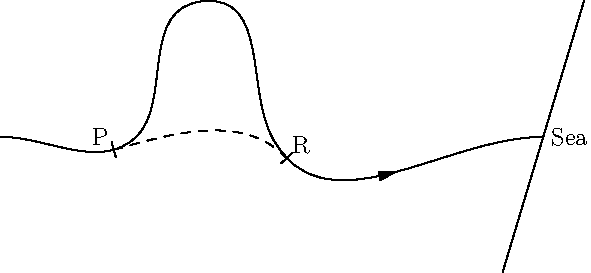
\includegraphics{cutoff.pdf}
    \caption{River cutoff}
    \label{fig:cutoff}
  \end{figure}
	Known:
	\begin{flalign*}
		So &= \SI{1e-4}{}&\\
		L_\text{0}  &= \SI{10}{\kilo\metre}&\\
		L_\text{1}  &= \SI{5}{\kilo\metre}&\\
    C &= \SI{50}{\m\tothe{0.5}\per\s}&\\
		b &= \SI{200}{\metre}&\\
		Q	&= \SI{1118}{\cubic\m\per\s}&
	\end{flalign*}

  \begin{exercise}
    Calculate the water depth at the locations P and R directly after the cut-off is realized ($t = 0$).
  \end{exercise}

  \begin{exercise}
    Make a plot of the situation before the cutoff and one for the situation after the cutoff
  \end{exercise}


\section{Hydraulic jump}
In this part we will work through an example which is quite instructive to understand how to impose boundary conditions and how backwaters interact at a hydraulic jump. A Hydraulic jump occurs when flow transitions from supercritical flow (i.e. $Fr>1$ to subcritical flow where $Fr<1$. 
We will consider a hydraulic jump in a horizontal flume, with a discharge of $Q=\SI{25}{\cubic\m\per\s}$, a width of $b=\SI{0.405}{\m}$, a roughness of $C=\SI{50}{\m\tothe{0.5}\per\s}$. The length of the flume $L=\SI{5}{\m}$. At the upstream side of the flume there is an undershot gate, that sets an upstream boundary condition. At the downstream side a weir forces a downstream boundary condition.

Now, this is interesting. Why do we have both an upstream and a downstream boundary condition? The reason is that upstream of the hydraulic jump and downstream of the hydraulic jump we have two backwater developing that interact at the jump. 

\begin{exercise}
  Construct two backwater objects to represent the two backwater. For now, assume there is no jump and that both backwaters extend over the entire flume. For the weir, assume that the flow becomes critical over the weir. Use a weir height of \SI{5}{\cm} and an undershot opening of \SI{3}{\cm}.
\end{exercise}

Now that you have constructed the two backwater, the question is: where does the hydraulic jump occur that makes the upstream backwater 'jump' to the downstream backwater. There is a very specific point where the jump will occur, and this point is determined by a momentum balance over a hydraulic jump. When worked out one can compute the depth  that would occur downstream of a jump ($a_\text{jump}$, given the upsteream depth ($a_1$) and froude number ($Fr_1$):
\begin{align*}
  a_\text{jump}=\dfrac{a_1}{2}(\sqrt{1+8Fr_1^2}-1)
\end{align*}
With the two backwaters that you calculated, you can now figure out where in theflume the hydraulic jump would occur such that the upstream backwater curve exactly results in the depth of the downstream hydraulic jump.

\begin{exercise}
  Determine the $x$ location in the flume where the jump would occur.
\end{exercise}

\begin{exercise}
  Adapt the ending coordinate of the two backwater you made earlier, such that they end at the hydraulic jump, and create a figure of the jump
\end{exercise}

\begin{exercise}
  Can you make the jump move left and right, by adjusting the weir and gate levels?
\end{exercise}

Of course, there are many simplifications in the calculations used above. To test the accuracy of your computation you will create a hydraulic jump in the laboratory, and as part of that practical you can compare the practical results with the results from your backwater calculations.

\printsolutions
\end{document}
